% ===========================================================================
\section{Supplementary Note: Road-Transport Air Pollutants (EMEP/EEA Tier~1)}
\label{sec:air}
% ===========================================================================

This note reports the FY2023--24 road air-pollutant estimate using the EMEP/EEA 2023 Tier~1 factors. Native pollutant masses remain separate from greenhouse-gas aggregates. The national release extends the same source methods through FY2024--25 with source-year activities and declared factor applicability.

\textbf{Fuel is the activity, and it reconciles to the controls by construction.}
Tier~1 exhaust factors are grams per kilogram of fuel; the fuel each vehicle class
burns is the OCAC Road control total for the year---the same panel the greenhouse-gas
side burns, net of the same household-generator carve-out---split between classes by
the fleet model's energy-weighted class shares. Modelled fuel therefore equals sold
fuel for every fuel in every year, the anchor the superseded diagnostic explicitly
lacked; the class \emph{split} still rides the fleet model, so composition remains the
sector's weakest axis while the fuel quantity is constrained. Four process families are
estimated as separate atoms: hot-plus-cold exhaust (fuel-based), evaporative petrol
NMVOC (per-vehicle-day, at the guidebook's 20--35\,\si{\celsius} daily temperature
range, on the fleet model's own active vehicle counts), and tyre-and-brake and
road-surface wear (per vehicle-kilometre). Black carbon is the guidebook's f-BC
fraction of exhaust \PM{}---a component of particulate mass, never additional---and
\SOtwo{} is sulfur stoichiometry under the declared per-year fuel-sulfur regime of
\texttt{data/activity/transport/fuel\_sulfur\_by\_year.csv} (diesel on the same cited
Euro-II/Euro-V mandate boundaries the railways layer burns). Where the guidebook
publishes no Tier~1 factor for a Pakistani cell, the bridge table
(\texttt{data/activity/transport/emep\_class\_map.csv}) declares a named proxy---light
CNG vehicles take the passenger-car LPG chemistry, petrol buses the light-commercial
petrol row---never a silent one.

\begin{table}[htbp]
\centering
\footnotesize
\begin{tabular}{@{}lr@{}}
\toprule
\textbf{Pollutant} & \textbf{Tier~1 (kt/yr)} \\
\midrule
CO                   & 1430.4 \\
NMVOC                &  535.1 \\
\NOx{}               &  172.1 \\
\SOtwo{}             &   12.2 \\
\PM{}                &    8.2 \\
Black carbon         &    2.0 \\
\NHthree{}           &    2.6 \\
\bottomrule
\end{tabular}
\caption{Road transport, FY2023--24, EMEP/EEA Tier~1 on OCAC-reconciled fuel, all
processes. NMVOC is non-methane VOC;
\NOx{} is NO$_2$-equivalent mass, the inventory-wide basis. \PM{} here is the PM$_{2.5}$
core (exhaust \PM{} is PM$_{2.5}$ by the chapter's own statement, plus the wear
processes' PM$_{2.5}$); the wear processes' coarser TSP and PM$_{10}$ strata are
supplemental beside it, contained not additive, and appear in the factor appendix. The native factor definitions remain documented by process.}
\label{tab:air}
\end{table}

\begin{figure}[htbp]
\centering
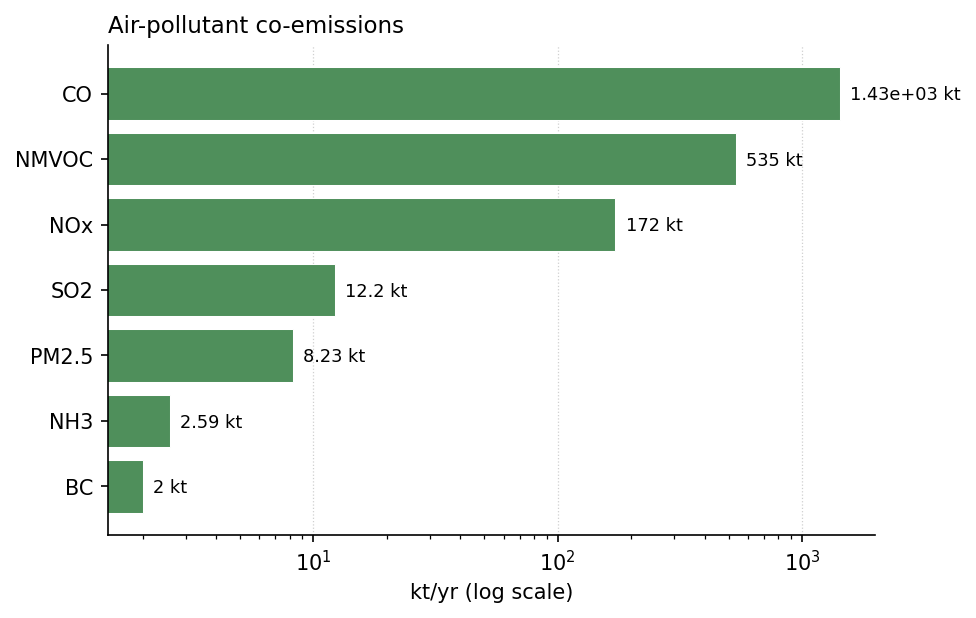
\includegraphics[width=\linewidth]{transport_air.png}
\caption{The Tier~1 layer, log axis: carbon monoxide exceeds black carbon by nearly
three orders of magnitude, which a linear axis cannot show. Wear TSP and PM$_{10}$
are excluded from the bars for the same containment reason the residential figure
excludes them.}
\label{fig:air}
\end{figure}

\subsection{Interpretation and conditional uncertainty}

A fuel balance constrains the amount consumed, but does not validate a transferred PM or NO$_x$ factor. Tier~1 fleet averages describe the guidebook's reference technologies and operating conditions; Pakistan's vehicle ages, two-wheelers, maintenance, catalysts and duty cycles remain unresolved. The source min--max factor spans and explicit technology cases therefore describe consequential assumptions rather than observed national fleet confidence limits. CNG-to-LPG chemistry and the petrol-bus class substitution remain named proxies. The conditional parameter ensemble retains its declared factor widths; separate technology and sulfur endpoints receive no assigned probability.

Exhaust, evaporation and wear retain distinct process records. Fuel-sales months support exhaust timing only as a combustion proxy. Evaporation and wear lack own-year monthly process evidence and use explicitly weaker allocation. Sulfur policy dates establish the specification scenario, not universal pump-level compliance. Primary particulate mass is an emission quantity; it does not provide ambient concentration, exposure or a health ranking.

\subsection{Limitations of this layer}

Tier~1 resolves fuel and broad vehicle category, not technology vintage, catalyst
penetration or after-treatment; the class split rides the fleet model's declared
intensity weights; the fuel-sulfur regime is declared from the import-mandate record,
not measured at the pump, and domestic-refinery waivers mean the post-2021 central
deliberately stays at the conservative pre-Euro-V specification; evaporative factors
assume the guidebook's hottest daily temperature band year-round; road-dust
resuspension stays out until a defensible local silt basis exists---a different claim,
recorded in the gap register to stop it riding in.
